\documentclass[tikz,convert={outfile=\jobname.svg}]{standalone}
\usepackage[arrowmos]{circuitikz}
\begin{document}
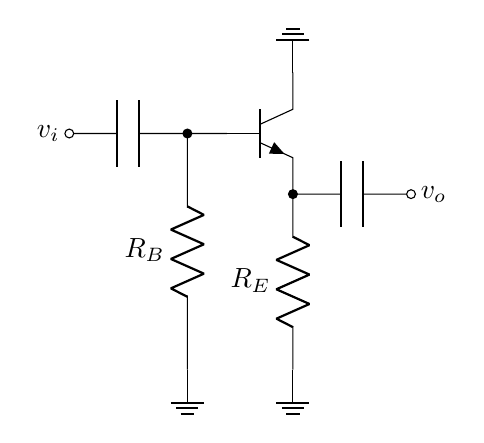
\begin{tikzpicture}
  \draw
  (0, 0) node[left] {$v_i$} to[C, o-*] (1.5, 0) to[R, l_=$R_B$] (1.5, -3) node[ground] (ground) {}
  (1.5, 0) -- (2, 0) node [npn, anchor=B] (npn) {}
  % https://tex.stackexchange.com/a/217501
  (npn.E) to[R, l_=$R_E$] (ground -| npn.E) node[ground] {}
  (npn.E) to[C, *-o] ++(1.5, 0) node[right] {$v_o$}
  (npn.C) node[ground, rotate=180] {}
  ;
\end{tikzpicture}
\end{document}
